\chapter{Wie du deine ToM+-Firmware aktualisierst}
\label{sec:update_procedure}

\section{Voraussetzungen vor dem Update}

ToM+ entwickelt sich ständig weiter, da ich fast täglich Vorschläge erhalte, um bestimmte Funktionen zu verbessern oder sogar neue, coole Features hinzuzufügen. Ich versuche, alle Ratschläge der Besitzer zu berücksichtigen, und diese Tipps und Ideen führen zu Firmware-Updates. Wenn du beim Fahren Fehler oder ungewöhnliches Verhalten bemerkst, melde diese bitte an mich, damit sie in Firmware-Patches behoben werden können. Wie ich eingangs erwähnt habe, wird ToM+ kontinuierlich verbessert – bleib also auf dem Laufenden\ldots

\subsection{Warum sollte ich aktualisieren?}

Nun, ein neues Update bedeutet neue Funktionen und Fehlerbehebungen. Warum solltest du also die alte Firmware-Version behalten, wenn du ganz einfach die neueste stabile Version installieren kannst? Es gibt also keinen Grund, dein ToM+ veraltet zu lassen, da das Software-Upgrade \textbf{für immer kostenlos} ist und dir beim Ausprobieren neuer Funktionen viel Freude und Spaß bringt. Letztendlich rate ich dir persönlich dazu, dein ToM+ auf dem neuesten Stand und sicherer zu halten.\\

Alle älteren Firmware-Versionen sind weiterhin im Twizy-Forum im ToM-Bereich (\url{https://www.twizy-forum.de/twiz-o-meter}) unter den Themen \textit{„[Twiz o'meter] Update auf Firmware x.x“} verfügbar. Tatsächlich erlaubt ToM+ bei Bedarf auch Downgrades.

\subsection{Was brauche ich für das Update?}

In den folgenden Abschnitten wird eine alternative Methode zum Aktualisieren beschrieben, die im Vergleich zur bereits in Abschnitt~\ref{sec:web_ota_update} besprochenen OTA-Methode deutlich zeitaufwendiger ist. Ich persönlich \textbf{empfehle die OTA-Methode}, da sie sicherer und einfacher durchzuführen ist, wenn man sich nicht besonders gut mit IT und Embedded Systems auskennt.\\

Wenn du dennoch davon überzeugt bist, die ToM+-Firmware mit der zweiten Methode zu aktualisieren, benötigst du ein paar Dinge, um das Update erfolgreich abzuschließen. Allererst benötigst du einen Computer; sowohl Desktop-PCs als auch Laptops sind für diese Aufgabe bestens geeignet.

Später werden wir sehen, wie du ToM+ mit dem Computer verbindest, um die neuen Update-Dateien darauf zu übertragen. Das zweite, was du besorgen musst, ist ein Micro-USB-Kabel – dasselbe, das gewöhnlich für aufladbare Geräte und ältere Smartphones verwendet wird. Zudem benötigst du eine microSD-Karte mit einer Speicherkapazität zwischen 8 und 32 GB.~Beispiele sind auf den Fotos unten zu sehen. Und natürlich benötigst du dein ToM+!

\begin{figure}[H]
    \centering
    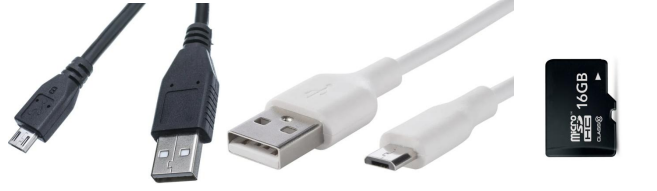
\includegraphics[width=0.8\textwidth]{figures/cables_sd_update.png}
    \caption{Micro-USB-Kabel und Beispiel einer microSD-Karte.}
\end{figure}


\subsection{Wie sehen die Update-Dateien aus?}
\label{sec:update_files}

Bevor du die Firmware aktualisierst, musst du natürlich die ZIP-Datei der gewünschten Version aus dem Twizy-Forum (wieder unter \url{https://www.twizy-forum.de/twiz-o-meter}) herunterladen.~Wahrscheinlich musst du dich im Forum registrieren, um Firmware-Dateien und Bilder zu sehen und herunterzuladen. Es ist eine wirklich tolle und aktive Community, daher empfehle ich ohnehin, Mitglied zu werden. Nach dem Entpacken der Dateien in den Ordner solltest du Folgendes erhalten:

\begin{figure}[H]
    \centering
    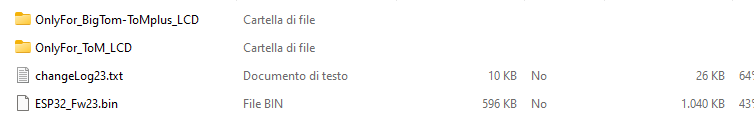
\includegraphics[width=1\textwidth]{figures/firmware_release_folder.png}
    \caption{Dateiliste des Firmware-Release-Ordners.}
\end{figure}

Zuerst bemerken wir eine Textdatei namens \textit{changeLog23.txt}, mit der die hinzugefügten Funktionen und behobenen Fehler der neuesten Firmware-Version nachverfolgt werden. Lies sie durch, wenn du neugierig bist, was es Neues gibt, oder wenn du zusätzliche Hilfe beim Update-Vorgang benötigst.\\

Als Nächstes gibt es zwei Ordner, die das \textbf{LCD-Display-Firmware}-Update im \textit{.tft}-Format enthalten. \textbf{Wähle die Version}, die für dein Gerät gemacht ist: den ersten Ordner, wenn du ein ToM+ oder ein BigToM hast (was ein größeres Display bedeutet), oder den anderen, wenn du ein traditionelles ToM hast oder das Twin ToM (kleinerer Bildschirm) aktualisieren möchtest. Dies ist ein entscheidender Schritt, da neue Icons und Grafiken sonst nicht zu deiner Displaygröße passen.\\

Die letzte Datei ist die Binärdatei \textit{ESP32\textunderscore Fw23.bin} für das \textbf{Blackbox-Update}. Stelle sicher, dass du alle diese Dateien hast, da du sie in den nächsten Schritten benötigst.

\subsection{Was sollte ich vor dem Update wissen?}

Bereiten wir nun unser ToM+ auf das Update vor, indem wir den \textbf{Schalter an der Blackbox auf OFF stellen}. Stelle sicher, dass er ausgeschaltet ist (\textit{d.\,h. Symbol 0 auf dem Schalter}), da du andernfalls schwerwiegende Probleme am ToM+ verursachen wirst.

Wenn dein Twizy also noch mit eingestecktem Schlüssel eingeschaltet ist, schalte ihn einfach komplett aus und ziehe den Zündschlüssel ab. Nach diesen einfachen Schritten bist du bereit für den Update-Vorgang. Denke jedoch daran, den in der Anleitung beschriebenen Schritten strikt zu folgen. Gehe nicht nach Gefühl vor, da du sonst riskierst, dein Gerät dauerhaft zu unbrauchbar zu machen.\\

Der Aktualisierungsvorgang ist recht einfach, und du musst sowohl die LCD-Firmware als auch die der Blackbox in genau dieser Reihenfolge aktualisieren. Wie das geht, sehen wir im nächsten Abschnitt.



\section{Aktualisieren der LCD-Firmware}

Das LCD-Display ist eines der wesentlichen Bauteile von ToM+, wie in den ersten beiden Kapiteln besprochen wurde, und muss aus diesem Grund ebenfalls aktualisiert werden. Neue Firmware bedeutet neue Icons und andere Layouts. Um die neuen Daten aufzuspielen, ist es unerlässlich, eine kleine \textbf{microSD-Karte} zu verwenden. Der SD-Kartensteckplatz des ToM+ befindet sich unter dem Display. Daher musst du es möglicherweise vorübergehend aus dem Handschuhfach nehmen, um besser daran arbeiten zu können, oder es einfach nach hinten kippen, um die Öffnung zu sehen.

\subsection{Vorbereiten der microSD-Karte}

Leider funktionieren nicht alle microSD-Karten mit dem Display, insbesondere neuere, die für Kameras entwickelt wurden. Bisher habe ich jedoch Class 10 HC-Karten von 8 bis 32 GB getestet, und diese scheinen gut zu funktionieren. Du kannst es aber gerne mit deiner eigenen Speicherkarte versuchen und prüfen, ob sie funktioniert.\\

Nachdem wir eine microSD-Karte ausgewählt haben, die eine Speicherkapazität \textbf{zwischen 8 und 32 GB} besitzen muss, müssen wir die LCD-Firmware darauf kopieren. Bevor wir die Datei darauf kopieren, müssen wir sicherstellen, dass sich keine anderen Dateien darauf befinden, da das Upgrade sonst nicht funktioniert.

Verschiebe daher alle Dateien auf deinen Computer und formatiere die microSD-Karte im \textbf{FAT32-Format}, wie ich es im Screenshot hier getan habe. Klicke dazu mit der rechten Maustaste auf das Kartensymbol in deinem Datei-Explorer und wähle die Option \textbf{„Formatieren…“} aus dem Kontextmenü.

\begin{figure}[H]
    \centering
    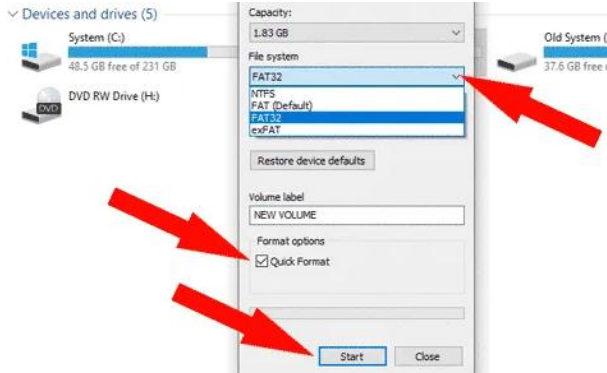
\includegraphics[width=0.7\textwidth]{figures/forma_sd_steps.png}
    \caption{Schritte zum Formatieren der microSD-Karte in FAT32.}
\end{figure}

Wie im Bild gezeigt, wähle das Dateisystem \textbf{FAT32}, aktiviere die Option \textbf{„Schnellformatierung“} und drücke die Schaltfläche \textbf{„Starten“}, um den Vorgang zu beginnen. Warte, bis der Vorgang abgeschlossen ist, und kopiere dann die \textit{.tft}-Datei aus dem ZIP-Ordner des Firmware-Releases, das du installieren möchtest, auf die Karte.


\subsection{Einsetzen der microSD-Karte}

Jetzt sind wir bereit, die microSD-Karte in den Steckplatz des LCD-Displays einzusetzen. Es kann hilfreich sein, eine Spitzzange zu verwenden, um die microSD-Karte vorsichtig einzuführen. Dies stellt sicher, dass du den internen SD-Kartensteckplatz genau triffst.\\

\textbf{WICHTIG!} Die microSD-Karte passt nur in einer Richtung in den Steckplatz: Die Kontaktseite muss zur Bildschirmoberfläche zeigen, wie im Bild dargestellt. Wenn sie nicht passt, wende keine Gewalt an! Versuche, sie umzudrehen.

Nachdem die microSD-Karte in den internen Steckplatz eingeführt wurde, drücke sie langsam in das Gehäuse, bis du ein „Klick“-Geräusch hörst. Das bedeutet, dass du die Zange sicher entfernen kannst, ohne dass die Karte im Gehäuse verloren geht.

\begin{figure}[H]
    \centering
    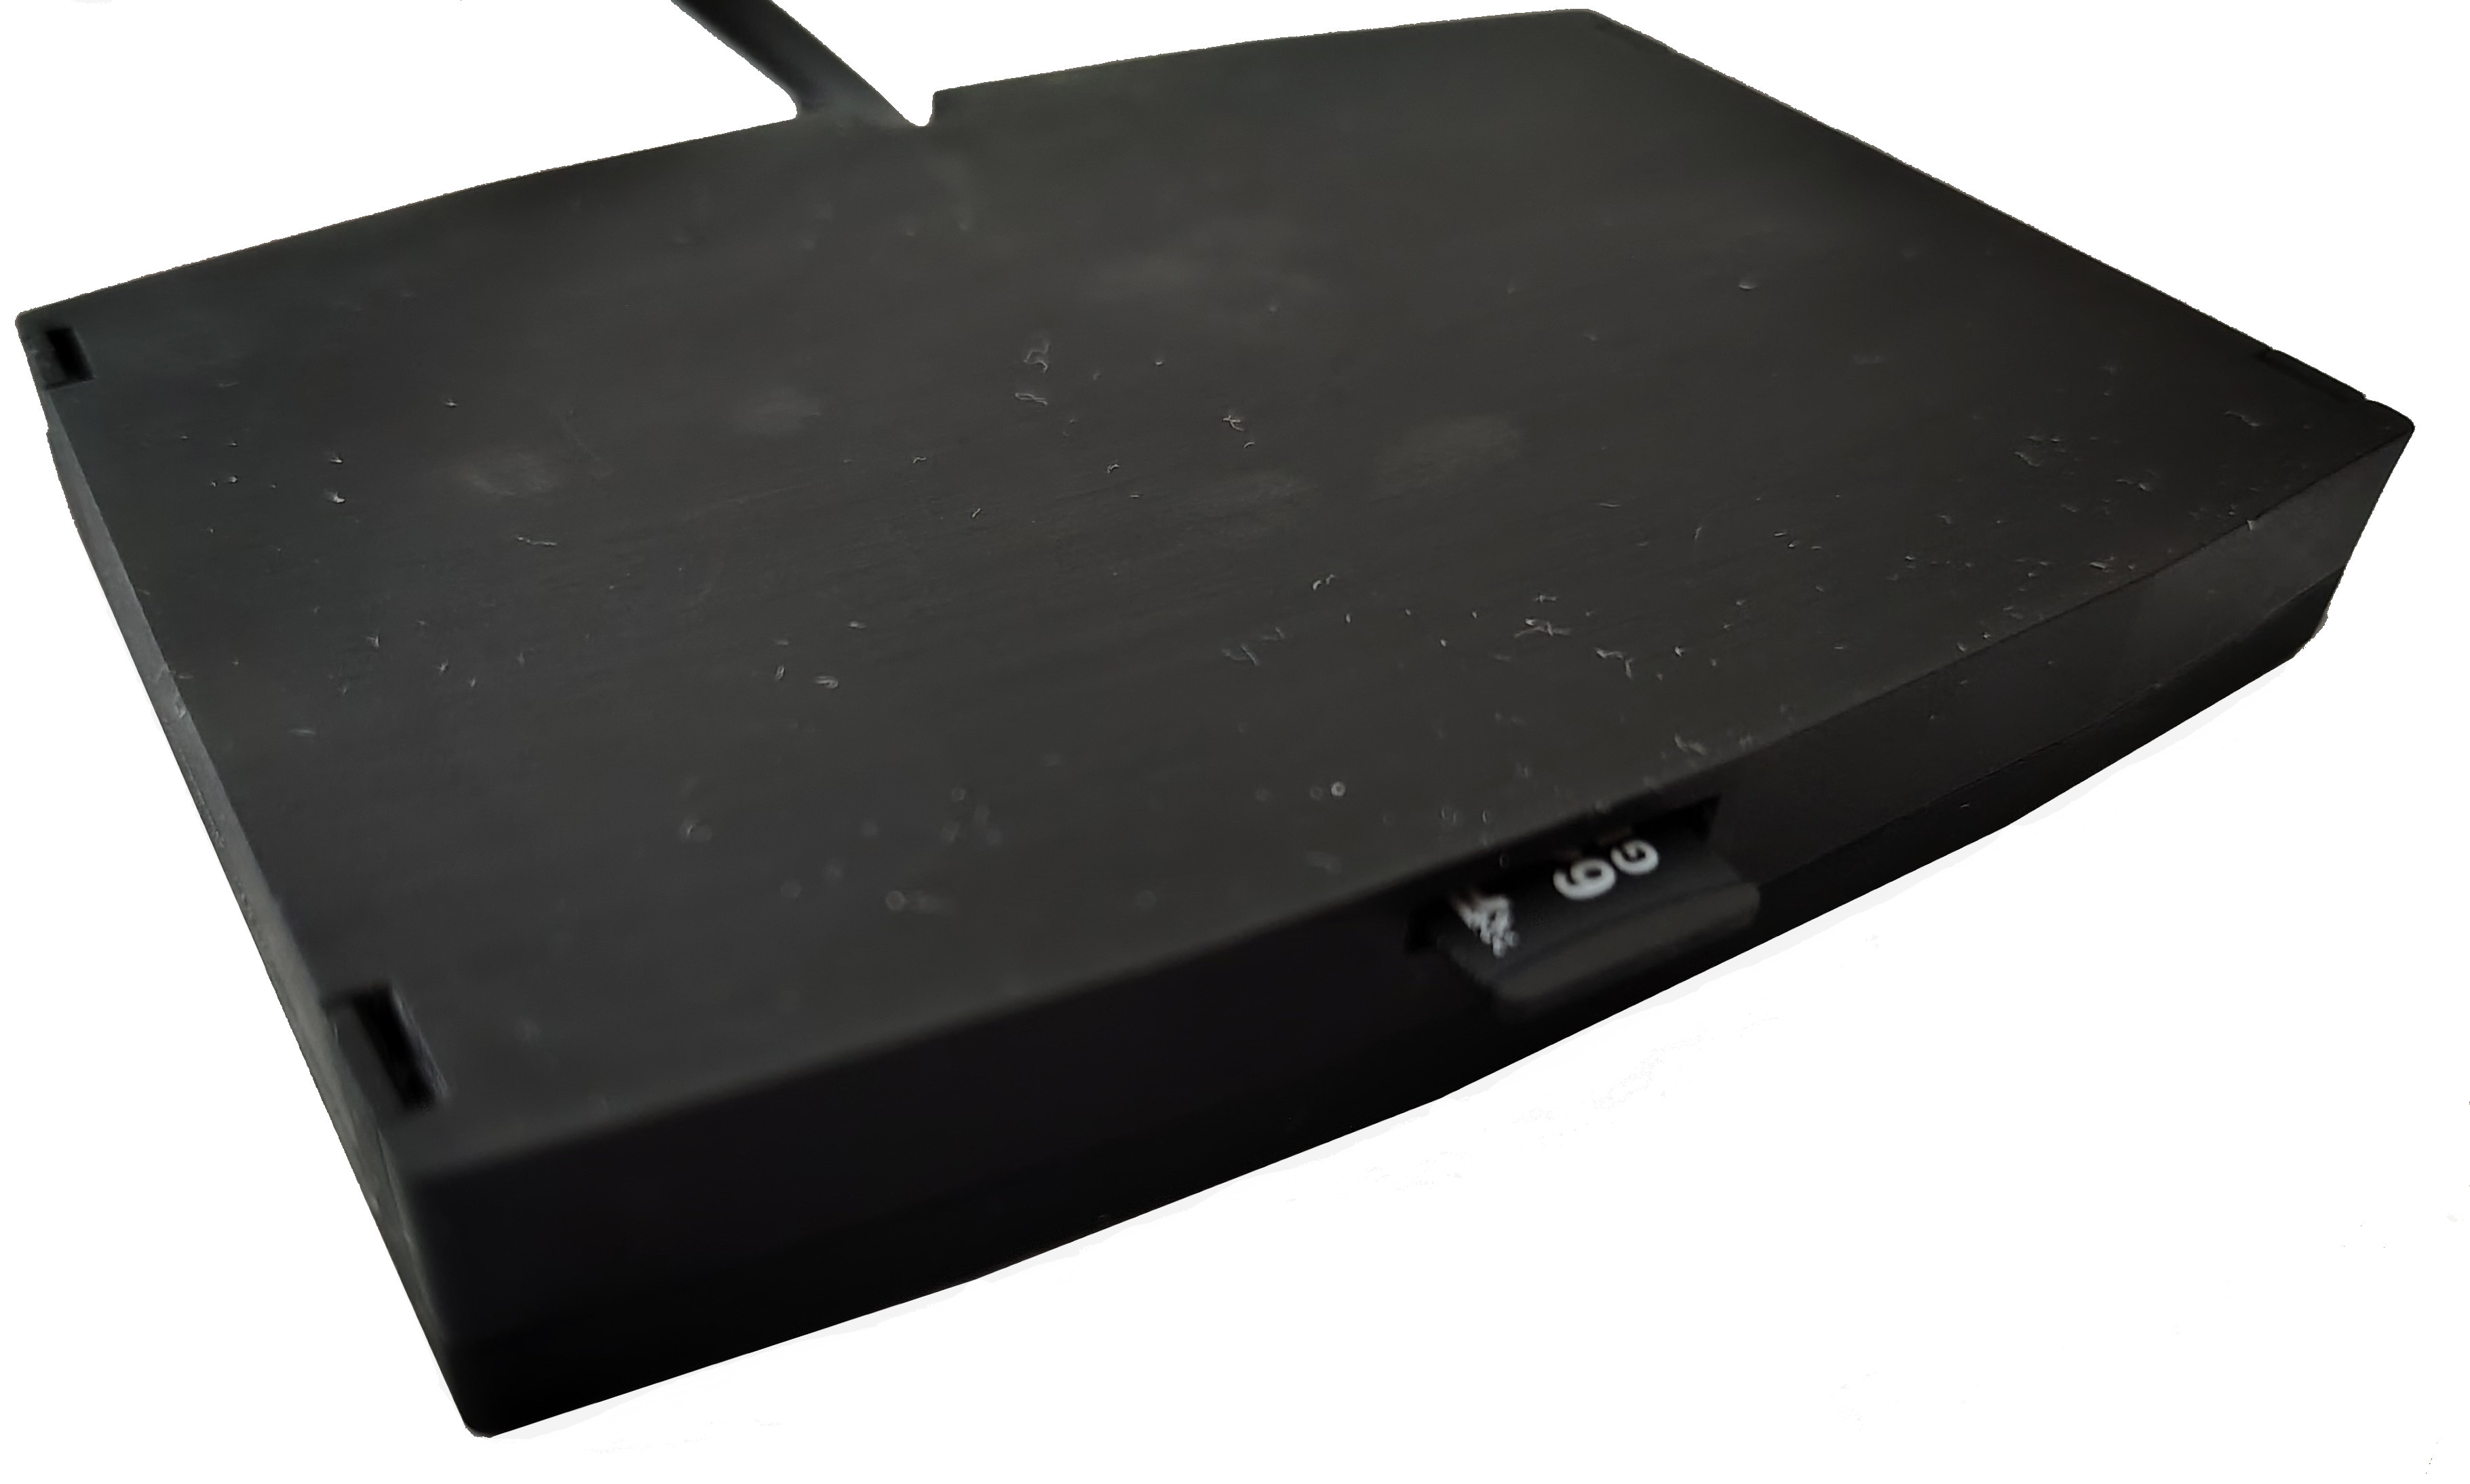
\includegraphics[width=0.6\textwidth]{figures/sd_insert.jpg}
    \caption{microSD-Karte in die Öffnung des Displays einsetzen.}
\end{figure}


\subsection{Der Ablauf des Updates}

Sobald die microSD-Karte eingesetzt ist, können wir mit dem Update-Ablauf fortfahren. Gehen wir nun zurück zum Twizy und schließen das Display wieder an die Blackbox an. Schalte dann das Display über den Schalter an der Blackbox ein (\textit{d.\,h. Symbol 1 auf dem Schalter}) und schalte erst danach deinen Twizy mit dem Zündschlüssel ein.

Warte, bis das LCD-Display den Aktualisierungsvorgang startet und der Fortschritt in Prozent angezeigt wird, wie in der Abbildung unten dargestellt (sowohl für das ToM+- als auch für das ToM-Display). Der Kopiervorgang von der microSD-Karte dauert in der Regel etwa eineinhalb Minuten.

\begin{figure}[ht]
    \centering

    \begin{subfigure}[t]{0.48\textwidth}
        \centering
        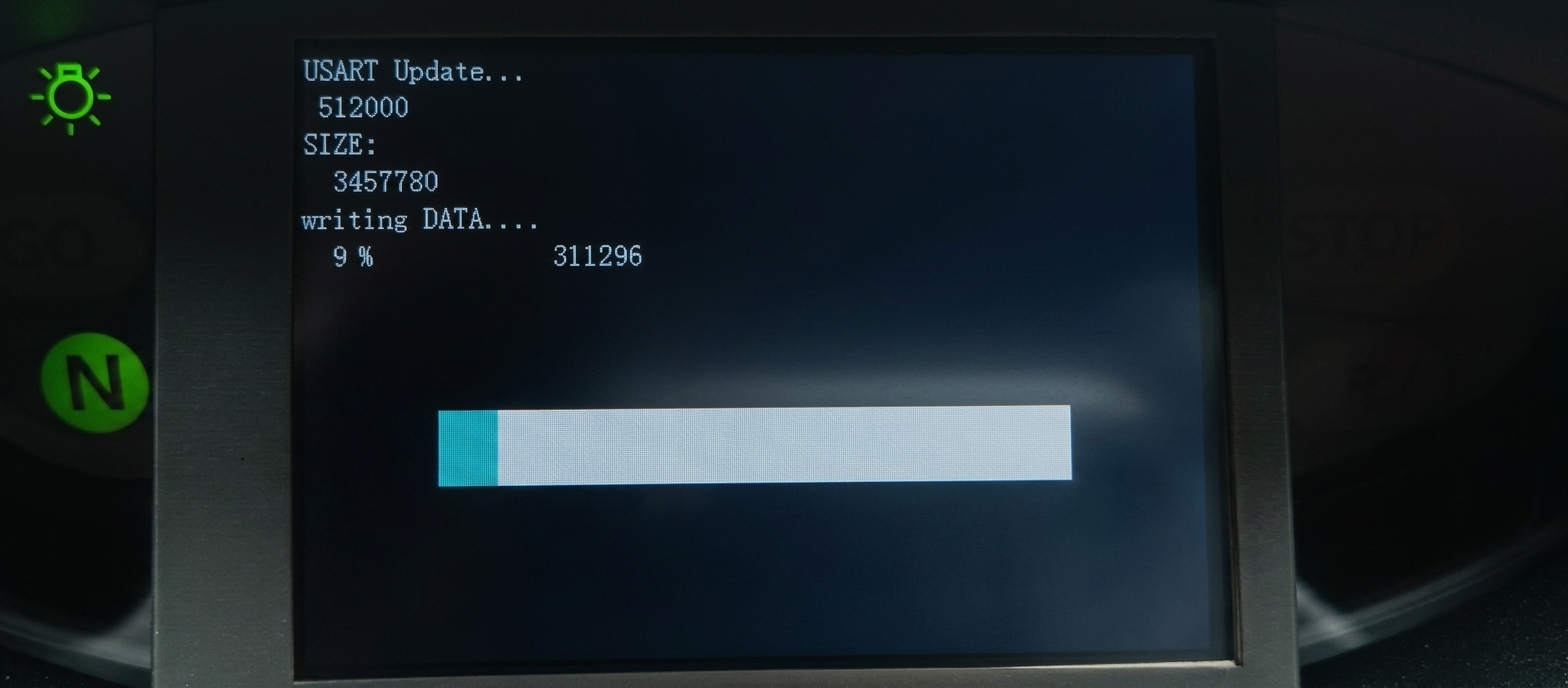
\includegraphics[width=\linewidth]{figures/update_screen_lcd.jpg}
        \caption{ToM+-Display-Update.}
    \end{subfigure}
    \hfill
    \begin{subfigure}[t]{0.48\textwidth}
        \centering
        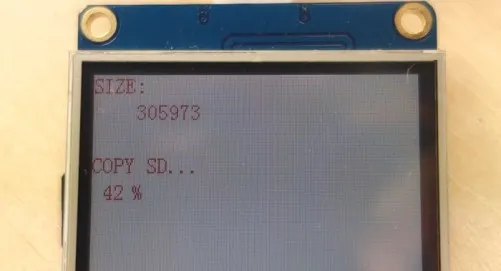
\includegraphics[width=\linewidth]{figures/copy_sd_card.png}
        \caption{ToM-Display-Update.}
    \end{subfigure}
\end{figure}

Sobald die Aktualisierung der LCD-Firmware erfolgreich abgeschlossen ist, siehst du diesen Bildschirm mit der Meldung \textbf{„Update Succeeded!“}. Nach dem Update das Gerät \textbf{NICHT} mit eingesteckter microSD-Karte einschalten! Jetzt können wir das Auto ausschalten und ToM+ über den Schalter an der Blackbox wieder auf OFF schalten.

Entferne dann die microSD-Karte, während das gesamte System ausgeschaltet ist, womit das LCD-Update abgeschlossen ist. \textbf{WICHTIG!} Wenn du die Karte entfernst, während ToM+ eingeschaltet ist, wirst du das Gerät dauerhaft unbrauchbar machen! Fahren wir danach, ohne den Zustand des Gesamtsystems zu verändern, mit dem Blackbox-Update fort, wie im nächsten Abschnitt beschrieben.



\section{Aktualisieren der Blackbox-Firmware (Windows)}

Die Blackbox ist die zweite wesentliche Komponente von ToM+ und bildet das Gehirn des gesamten Systems. Wenn wir nur das Display aktualisieren, weiß die Blackbox nicht, wofür die neuen Icons gedacht sind, was zu Kommunikationsfehlern führt.

Daher ist es entscheidend, die neue Firmware auch auf der Hauptplatine von ToM+ zu installieren. Dazu benötigen wir die microSD-Karte nicht mehr, sondern verwenden das zuvor vorbereitete Micro-USB-Kabel und den Computer. Wir werden die Firmware direkt auf das ESP32-Board flashen, um die neue Software zu installieren.


\subsection{Vorbereiten des Computers}

Bevor wir das Kabel an den Computer anschließen, müssen wir einige Programme installieren, damit alles ordnungsgemäß funktioniert. Das \textbf{ESP32-Board} benötigt Treiber, um vom Betriebssystem erkannt zu werden. Wir laden diese direkt von der offiziellen Website herunter.

Auf der Download-Seite der \href{https://www.silabs.com/software-and-tools/usb-to-uart-bridge-vcp-drivers?tab=downloads}{Silicon Labs-Website} müssen wir unsere Betriebssystemversion auswählen, wie im Screenshot unten zu sehen ist.

\begin{figure}[H]
    \centering
    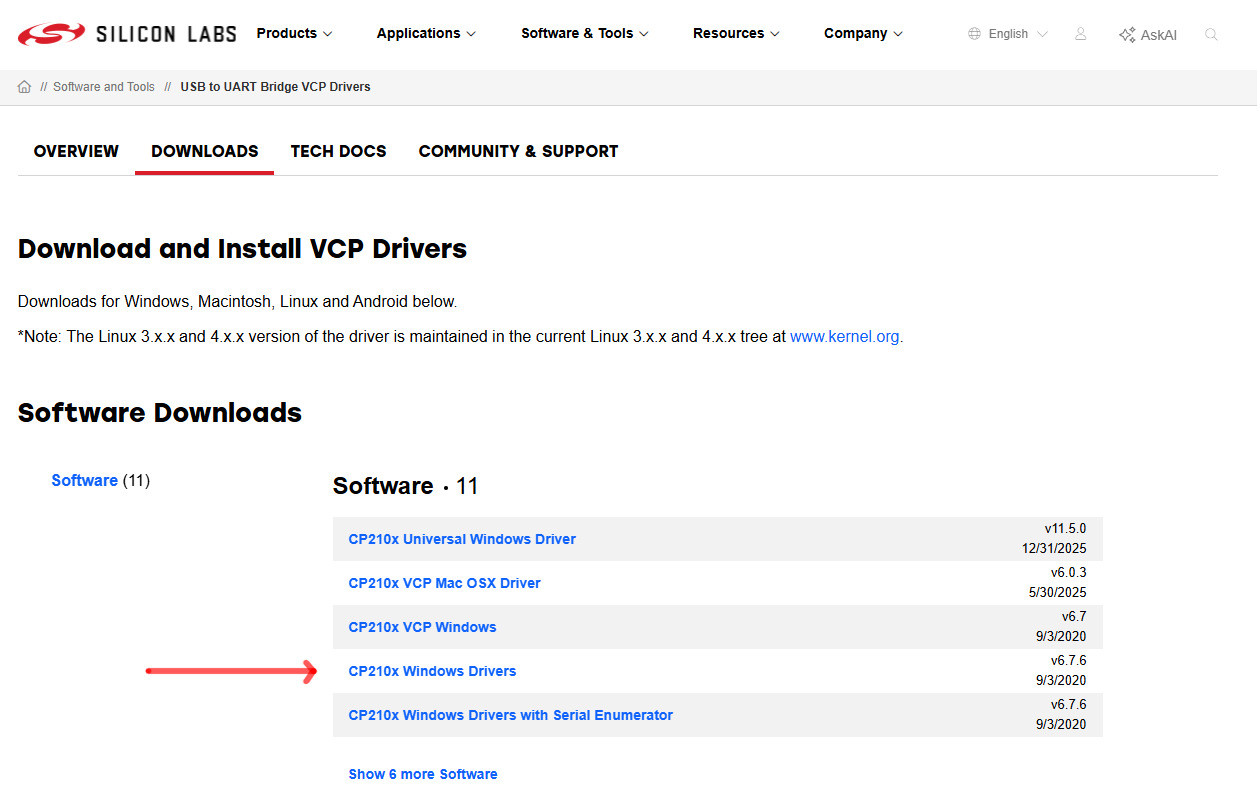
\includegraphics[width=1\textwidth]{figures/driver_download.png}
    \caption{Treiber-Downloadseite bei Silicon Labs.}
\end{figure}

Da dieser Abschnitt der Anleitung speziell für Windows-Betriebssysteme gilt, laden wir das Paket \textit{„CP210x Windows Drivers“} herunter, indem wir auf den im Bild oben gelb markierten Link klicken.

Die heruntergeladene Datei ist ein ZIP-Ordner, der gewöhnlich \textit{„CP210x\textunderscore Windows\textunderscore Drivers.zip“} heißt und in dem sich einige Ordner und Dateien befinden. Im Screenshot unten sind alle üblicherweise im ZIP-Ordner enthaltenen Dateien aufgelistet.

\begin{figure}[H]
    \centering
    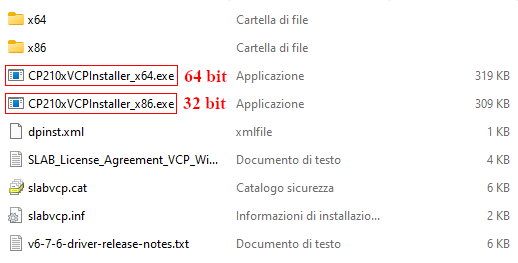
\includegraphics[width=0.7\textwidth]{figures/driver_folder.png}
    \caption{Inhalt des Treiber-ZIP-Ordners.}
\end{figure}

Entpacke alle Dateien in einen temporären Ordner auf deinem Desktop. Nun ist es wichtig, die richtige \textit{„.exe“}-Datei für die Installation der Treiber auszuführen. Wenn dein Betriebssystem 64-Bit ist (bei den meisten Computern), führst du die Datei \textit{CP210xVCPInstaller\textunderscore x64.exe} aus, andernfalls ist die zweite \textit{„.exe“}-Datei die passende, wie im Bild gezeigt.

Stelle sicher, dass du die ausführbare Datei mit Administratorrechten startest, indem du mit der rechten Maustaste darauf klickst und die Option \textbf{„Als Administrator ausführen“} wählst. Falls du dazu aufgefordert wirst, erlaube dem Programm, Administratoraktionen auf deinem Computer auszuführen, da der Treiber-Installationsprozess sonst nicht startet.

\begin{figure}[ht]
    \centering

    \begin{subfigure}[t]{0.48\textwidth}
        \centering
        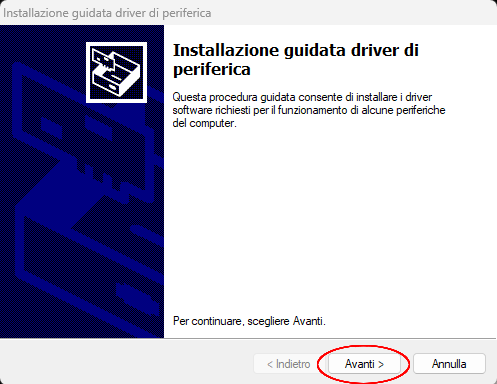
\includegraphics[width=\linewidth]{figures/wizard_step1.png}
        \caption{Erster Schritt: „Weiter“ drücken.}
    \end{subfigure}
    \hfill
    \begin{subfigure}[t]{0.48\textwidth}
        \centering
        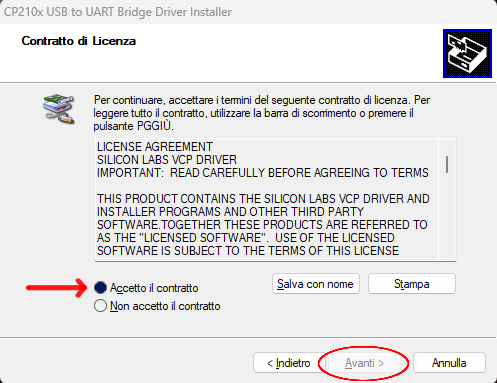
\includegraphics[width=\linewidth]{figures/wizard_step2.png}
        \caption{Zweiter Schritt: „Akzeptieren“ und „Weiter“.}
    \end{subfigure}
\end{figure}

Sobald das Installationsprogramm startet, siehst du ein Fenster wie das auf der linken Seite. Dies ist ein Assistent zur Installation der Treiber, die erforderlich sind, damit dein Computer die Blackbox erkennt. Drücke nun die Schaltfläche \textbf{„Weiter“}, wie hier gezeigt, um den Vorgang zu starten.\\

Das nächste Fenster, das du voraussichtlich sehen wirst, ist das auf der rechten Seite. Hier musst du die Lizenz akzeptieren, indem du die erste Option \textbf{„Lizenz akzeptieren“} auswählst. Anschließend kannst du auf die Schaltfläche \textbf{„Weiter“} drücken und das Kopieren der Treiber in den richtigen Systemordner starten: Warte, bis der Kopiervorgang abgeschlossen ist.

Wenn das Kopieren beendet ist, ist die Installation der CP210X-Treiber abgeschlossen und du kannst die Blackbox sicher an deinen Computer anschließen. Drücke nun die Schaltfläche \textbf{„Fertigstellen“}, um das Fenster zu schließen.\\

Stelle vor allen weiteren Schritten sicher, dass der Schalter an der ToM+-Blackbox auf OFF steht (\textit{d.\,h. Symbol 0 auf dem Schalter}). Der Twizy muss ebenfalls ausgeschaltet sein, denn wenn du versuchst, das Kabel an deinen PC anzuschließen, während ToM+ noch vom Fahrzeug mit Strom versorgt wird, vermischst du die Stromversorgungen (5V und 12V), was ToM+ definitiv beschädigen würde.

\begin{figure}[H]
    \centering
    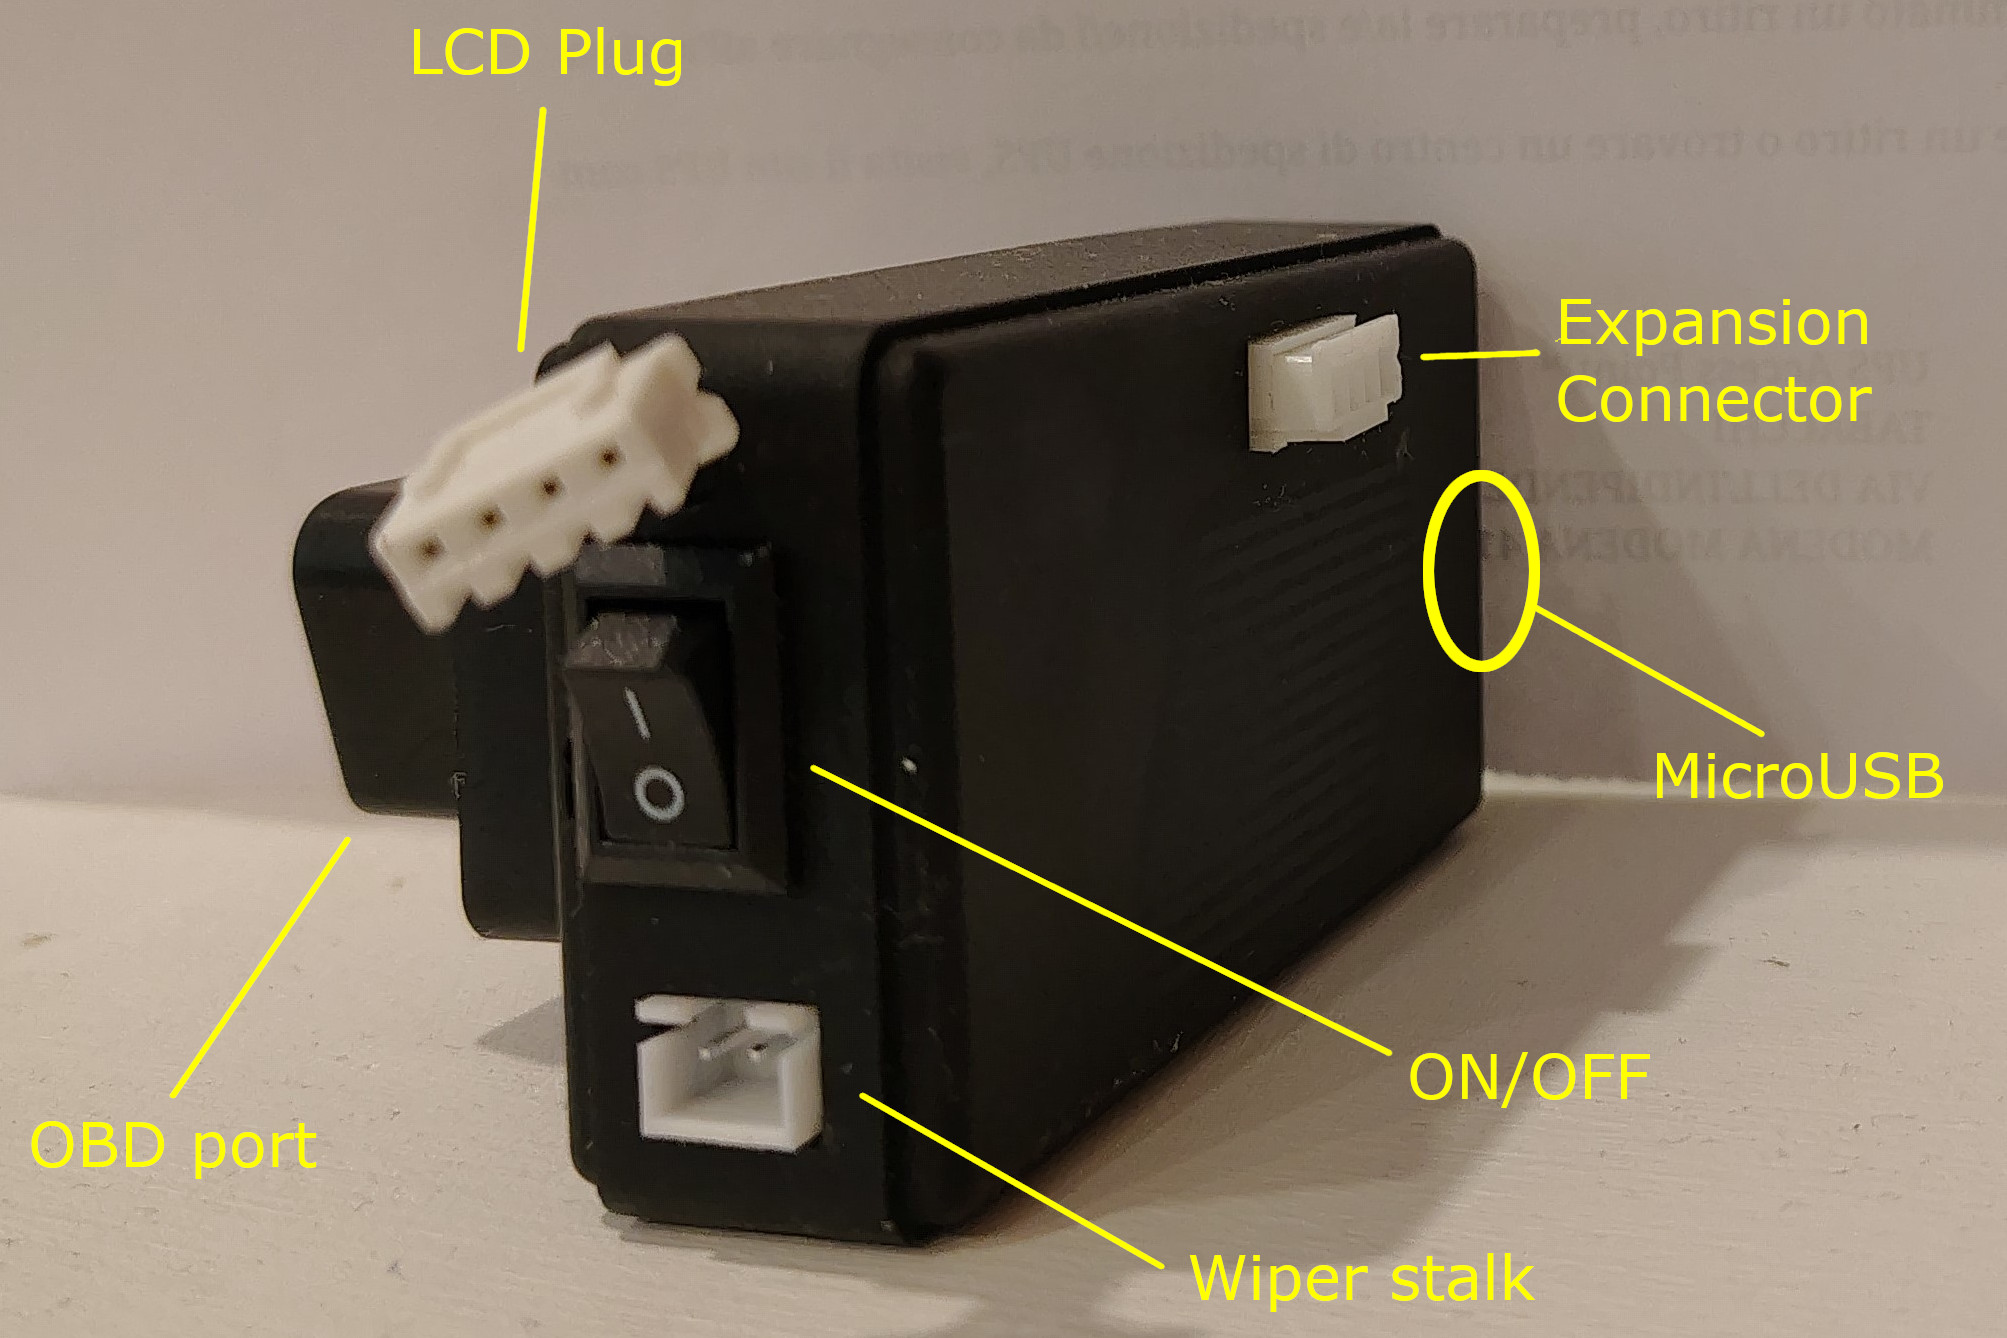
\includegraphics[width=0.6\textwidth]{figures/black_box.jpg}
    \caption{Die Komponenten der Blackbox.}\label{fig:black_box_labels}
\end{figure}

Die Blackbox verfügt auf der Rückseite über einen kleinen Micro-USB-Anschluss, wie im Bild oben zu sehen ist. Schließe also die Micro-USB-Seite des Kabels an die Blackbox an. Verbinde danach die USB-Seite des Kabels mit einem freien USB-Anschluss deines Computers.

\textbf{WICHTIG!} Beide Seiten des Kabels passen nur in einer Richtung in die entsprechenden Buchsen. Wende daher keine Gewalt an, da du sonst den Anschluss des ToM+ oder deines Computers beschädigen könntest. Versuche, den Stecker umzudrehen, und prüfe, ob es so passt.\\

Nun sollte der Computer das ESP32-Board der Blackbox erkennen, sofern du die Treiber ordnungsgemäß installiert hast. Um dies zu überprüfen, suche auf deinem PC nach der App \textbf{„Geräte-Manager“} und starte sie.

Nun sollte sich ein Fenster öffnen, das wie in der Abbildung unten aussieht. Suche die Zeile \textbf{„Anschlüsse (COM \& LPT)“} mit dem Steckersymbol und doppelklicke darauf, um die Liste aller seriellen Geräte zu öffnen. Suche, wie im Screenshot gezeigt, nach \textit{„Silicon Labs CP210x to UART Bridge (COMx)“} und notiere dir die COM-Nummer (im Beispiel \textbf{COM8}). Diese Nummer wird im nächsten Schritt benötigt, damit der PC weiß, wohin die neue Firmware-Version hochgeladen werden soll. Setzen wir diesen Vorgang fort\ldots

\begin{figure}[H]
    \centering
    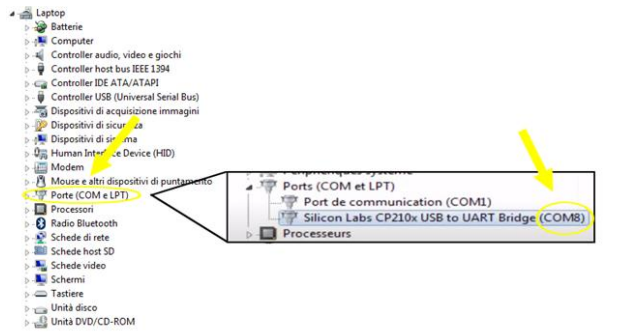
\includegraphics[width=0.8\textwidth]{figures/device_manager.png}
    \caption{Geräte-Manager UART serielle Schnittstelle (COM8).}
\end{figure}

Besuche die \href{https://www.espressif.com/en/support/download/other-tools}{offizielle ESP32-Website}, um ein Tool herunterzuladen, das wir zum Flashen der Firmware auf unsere Blackbox-Platine benötigen. Suche nach \textbf{„Flash Download Tools“} und drücke die Schaltfläche wie im Bild gezeigt. Suche dann auf der Seite nach den \textit{„Flash Download Tools“} mit dem Speichern-Symbol und klicke darauf.

Dadurch wird ein ZIP-Ordner namens \textit{„flash\textunderscore download\textunderscore tool\textunderscore x.x.x.zip“} heruntergeladen, wobei die „x“-Symbole durch die Versionsbezeichnung ersetzt werden (in diesem Beispiel \textbf{V3.9.11}). Beim Öffnen des heruntergeladenen ZIP-Ordners wirst du feststellen, dass sich darin ein weiterer Ordner befindet. Entpacke diesen auf deinen Desktop oder an einen beliebigen Ort und öffne ihn. Die darin enthaltenen Dateien entsprechen in der Regel den im Screenshot unten aufgelisteten.

\begin{figure}[H]
    \centering
    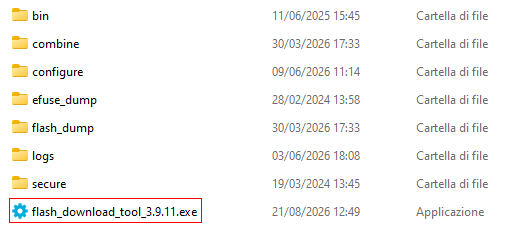
\includegraphics[width=0.7\textwidth]{figures/esptool_folder.png}
    \caption{Inhalt des Flash-Tools-ZIP-Ordners.}
\end{figure}

Wähle die Datei \textit{„flash\textunderscore download\textunderscore tool\textunderscore 3.9.11.exe“} (oder die entsprechende heruntergeladene Version) aus und führe sie mit Administratorrechten aus, indem du mit der rechten Maustaste auf die Datei klickst und die Option \textbf{„Als Administrator ausführen“} wählst. Falls du dazu aufgefordert wirst, erlaube der ausführbaren Datei die Durchführung von Aktionen auf deinem Computer.\\

Sobald das Programm gestartet ist, sollte sich ein Terminal-Fenster öffnen, das nach einigen Sekunden die Benutzeroberfläche startet. Sie sollte so aussehen wie im ersten Beispiel hier gezeigt. Du musst den \textbf{„ChipType“} auf \textit{„ESP32“} ändern, wie im zweiten Schritt unten dargestellt. Lass den Rest unverändert und drücke die Schaltfläche \textbf{„OK“}.

\begin{figure}[H]
    \centering
    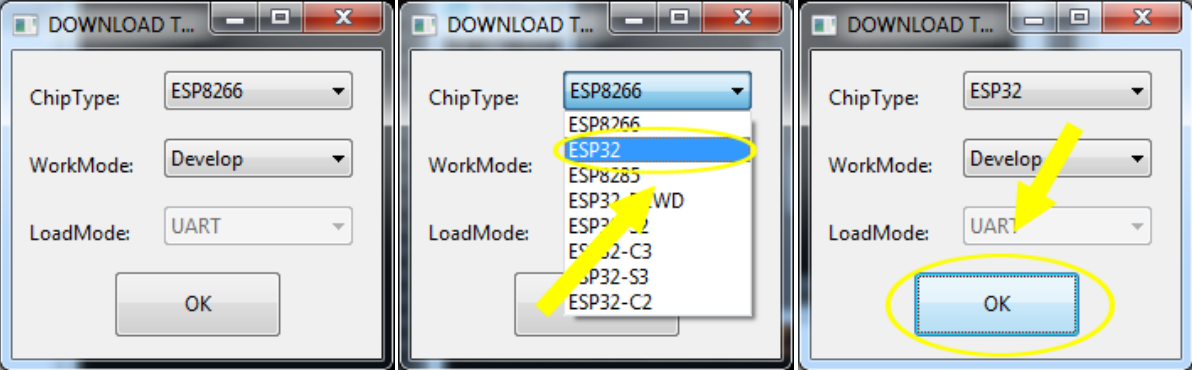
\includegraphics[width=0.85\textwidth]{figures/launching_flashtool.png}
    \caption{ESP32-Hauptplatine im Auswahldialog auswählen.}
\end{figure}


\subsection{Der Ablauf des Updates}

Sobald du die Schaltfläche \textbf{„OK“} drückst, öffnet sich ein Fenster mit dem Titel \textit{„ESP32 DOWNLOAD TOOL“}. Entpacke nun die Binärdatei (mit der Endung \textit{.bin}), die dem ToM+-Firmware-Release-ZIP beiliegt, wie in Abschnitt~\ref{sec:update_files} beschrieben.

Drücke dann die im ersten Bild gezeigte Schaltfläche \textbf{„…“} und wähle den Pfad der \textit{„.bin“}-Datei aus. Sobald du das getan hast, klicke auf die Schaltfläche \textbf{„Öffnen“}, woraufhin in der ersten Zeile ein grüner Eintrag mit dem gerade bestätigten Pfad erscheint.

Fahre fort, indem du das \textbf{Kontrollkästchen neben der ersten Zeile aktivierst}, um die Firmware auszuwählen, die du hochladen möchtest. Gib dann in das im zweiten Bild gezeigte Textfeld diese Zeichenfolge ein: \textbf{0$\times$10000} (mit vier Nullen). Dies stellt die Speicherstartadresse dar, an der die Firmware-Dateien abgelegt werden.

Nun folgt der letzte Konfigurationsschritt: Wähle die COM-Nummer über das Auswahlfeld in der unteren rechten Ecke. Stelle sicher, dass du den richtigen COM-Port auswählst, den wir uns zuvor im \textbf{Geräte-Manager} notiert haben.

\begin{figure}[H]
    \centering
    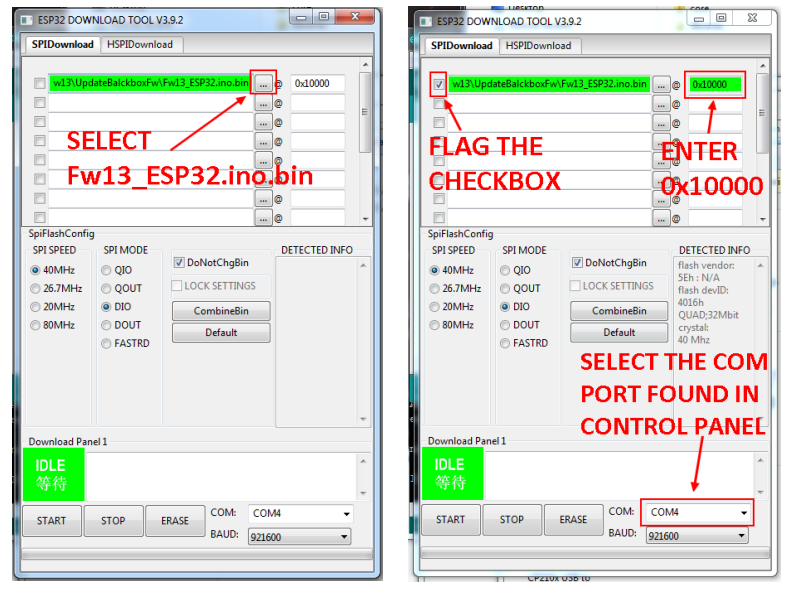
\includegraphics[width=1\textwidth]{figures/flashtool_page.png}
    \caption{Konfigurationsschritte im ESP32 Download Tool.}
\end{figure}

Starte nun das Update, indem du auf die Schaltfläche \textbf{„START“} drückst, wie im ersten Bild gezeigt. Am unteren Rand des Fensters erscheint ein grüner Fortschrittsbalken; der gesamte Vorgang dauert in der Regel ein paar Minuten.

Sobald der Upload abgeschlossen ist, siehst du die Meldung \textbf{„FINISH“} im grünen Feld in der linken unteren Ecke, wie im Bild gezeigt. Als zusätzliche Bestätigung ist der Fortschrittsbalken voll – das Update ist nun abgeschlossen.

\begin{figure}[H]
    \centering
    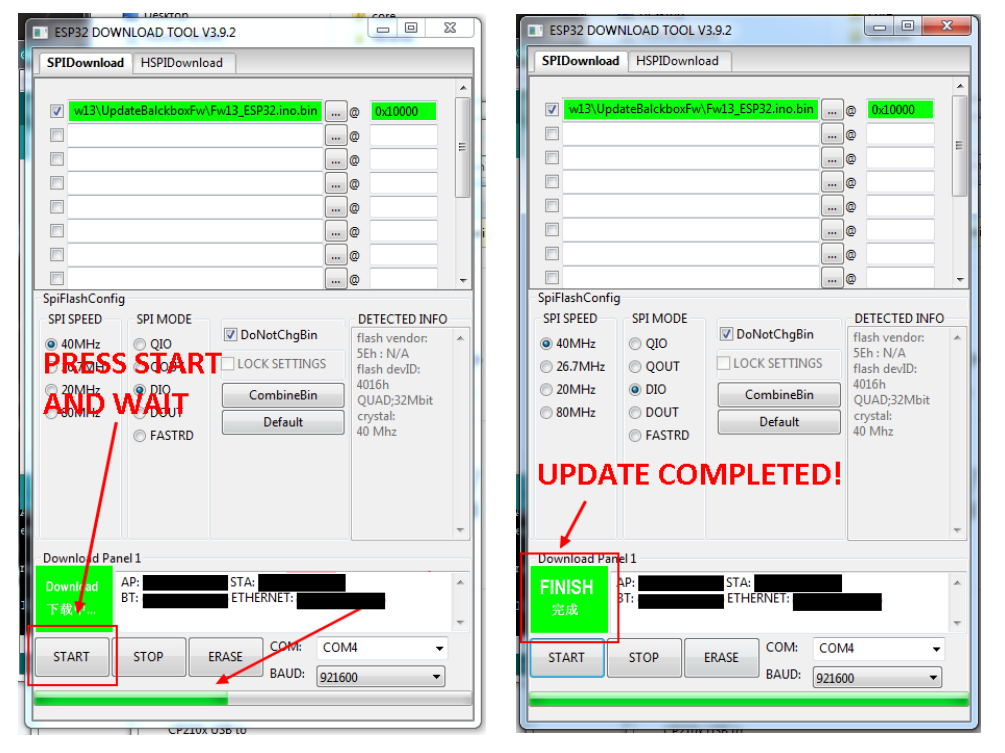
\includegraphics[width=1\textwidth]{figures/flashtool_page2.png}
    \caption{ESP32 Download Tool schließt das Update ab.}
\end{figure}

Schließe nun dieses Fenster. Anschließend kannst du das Kabel sicher von deinem PC und vom ToM+ trennen. Erst nach diesen Schritten kannst du die normale Stromversorgung des ToM+ wiederherstellen, indem du den Schalter in den Zustand 1 bringst und deinen Twizy mit dem Zündschlüssel einschaltest.

Um deine vorherigen Konfigurationen wiederherzustellen, rufe die ToM+-Einstellungsseite auf, indem du auf die drei Punkte in der oberen rechten Ecke drückst, und drücke dann die Beenden-Taste, ohne etwas zu ändern. Auf diese Weise wird die im Blackbox-Speicher gespeicherte Datenstruktur aktualisiert und deine Einstellungen sind wieder vorhanden.\\

\textbf{Herzlichen Glückwunsch!} Du hast den gesamten Update-Vorgang abgeschlossen. Genieße nun die neue Firmware und denke daran, mir Fehler oder Probleme per privater Nachricht zu melden, eventuell mit einem beigefügten Bild.


\clearpage

\section{Aktualisieren der Blackbox (Unix)}

Die Blackbox ist die zweite wesentliche Komponente von ToM+ und bildet das Gehirn des gesamten Systems. Wenn wir nur das Display aktualisieren, weiß die Blackbox nicht, wofür die neuen Icons gedacht sind, was zu Kommunikationsfehlern führt.

Daher ist es entscheidend, die neue Firmware auch auf der Hauptplatine von ToM+ zu installieren. Dazu benötigen wir die microSD-Karte nicht mehr, sondern verwenden das zuvor vorbereitete Micro-USB-Kabel und den Computer. Wir werden die Firmware direkt auf das ESP32-Board flashen, um die neue Software zu installieren.

Stelle vor allen weiteren Schritten den Schalter der ToM+-Blackbox auf OFF (\textit{d.\,h. Symbol 0 darauf}) und schalte auch deinen Twizy aus. Dies ist ein wichtiger Schritt, der strikt befolgt werden muss, um Schäden am Gerät zu vermeiden.

\subsection{Vorbereiten des Computers}

Lade den im Firmware-Release-Beitrag angehängten ToM+-Firmware-Update-Ordner herunter. Entpacke nun die im ToM+-Firmware-Release-ZIP enthaltene Binärdatei (Endung \textit{.bin}), wie in Abschnitt~\ref{sec:update_files} beschrieben. Die Datei heißt in der Regel \textit{„FwXX\textunderscore ESP32.bin“}, wobei das Symbol \textit{„XX“} durch die Versionsnummer ersetzt wird, zum Beispiel \textit{„23“}.\\

\textbf{Haftungsausschluss:} \textit{Dieser Blackbox-Vorgang wurde unter Ubuntu 20.04 getestet (hoffe, er funktioniert auch mit anderen Unix-Distributionen). Schließe die Blackbox erst an, wenn du ausdrücklich dazu aufgefordert wirst}.\\

Nun müssen wir das Paket esptool installieren, um die neue Firmware auf die Blackbox zu flashen. Führe dies entweder über die grafische Benutzeroberfläche der Paketverwaltung deiner Unix-Distribution aus oder mit dem entsprechenden Befehl im Terminal. Zum Beispiel \textit{„sudo apt-get esptool“}, wie im Bild gezeigt. Gib bei Aufforderung das Passwort des Sudo-Benutzers ein, drücke EINGABE und warte.

\begin{figure}[H]
    \centering
    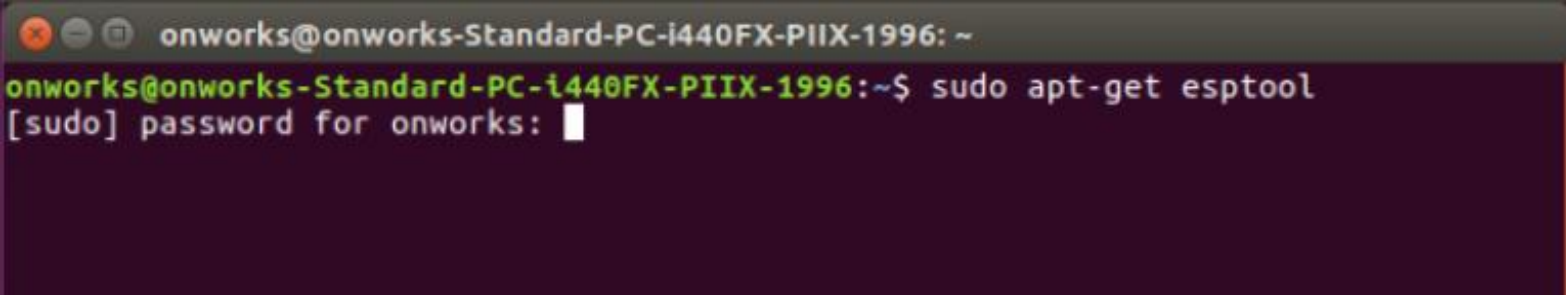
\includegraphics[width=1\textwidth]{figures/apt_get_esptool.png}
    \caption{Installation des esptool-Pakets unter Ubuntu.}
\end{figure}

Als Nächstes musst du Python installieren, falls du es noch nicht installiert hast, da das esptool in der Sprache Python geschrieben ist. Gib daher den Befehl \textit{„sudo apt-get python“} ein, wie im Bild gezeigt. Gib bei Aufforderung erneut das Passwort des Sudo-Benutzers ein, drücke EINGABE und warte.

\begin{figure}[H]
    \centering
    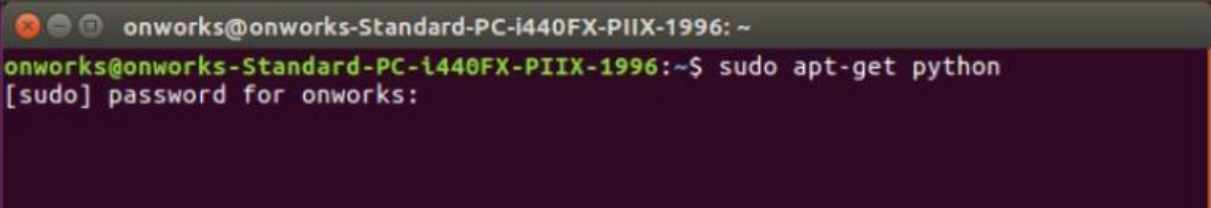
\includegraphics[width=1\textwidth]{figures/apt_get_python.png}
    \caption{Installation des Python-Pakets unter Ubuntu.}
\end{figure}

Sobald beide Pakete installiert sind, gib \textit{„sudo tail -f /var/log/messages“} im Terminal ein, wie im Bild gezeigt, um die Logdatei in Echtzeit zu überwachen. Diese zeigt an, welchem COM-Port die Blackbox vom Betriebssystem zugewiesen wird.~Gib bei Aufforderung das Passwort des Sudo-Benutzers ein und drücke EINGABE.~\textbf{Jetzt können wir die Blackbox anschließen}.

\begin{figure}[H]
    \centering
    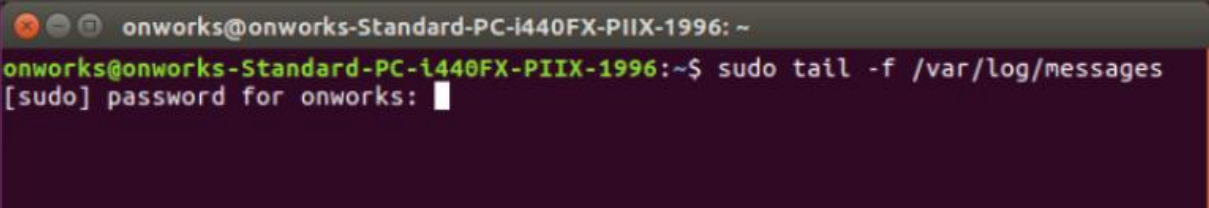
\includegraphics[width=1\textwidth]{figures/tail_com.png}
    \caption{Echtzeit-Überwachung der COM-Verbindungen.}
\end{figure}

Die Blackbox verfügt auf der Rückseite über einen kleinen Micro-USB-Anschluss, wie in Abbildung~\ref{fig:black_box_labels} zu sehen ist. Schließe also die Micro-USB-Seite des Kabels an die Blackbox an. Verbinde danach die USB-Seite des Kabels mit einem freien USB-Anschluss deines Computers.

\textbf{WICHTIG!} Beide Seiten des Kabels passen nur in einer Richtung in die entsprechenden Buchsen. Wende daher keine Gewalt an, da du sonst den Anschluss des ToM+ oder deines Computers beschädigen könntest. Versuche, den Stecker umzudrehen, und prüfe, ob es so passt.\\

Sobald du die Blackbox an den Computer anschließt, solltest du eine Ausgabe erhalten, die der hier im Codeblock gezeigten ähnelt.

\begin{lstlisting}[language=bash]
Oct 15 11:05:14 Kubuntu2004 kernel: [ 172.232228] usb 1-3: new full-speed USB
device number 3 using xhci_hcd
Oct 15 11:05:14 Kubuntu2004 kernel: [ 172.423441] usb 1-3: New USB device found,
idVendor=10c4, idProduct=ea60, bcdDevice= 1.00
Oct 15 11:05:14 Kubuntu2004 kernel: [ 172.423453] usb 1-3: New USB device
strings: Mfr=1, Product=2, SerialNumber=3
Oct 15 11:05:14 Kubuntu2004 kernel: [ 172.423457] usb 1-3: Product: CP2102 USB
to UART Bridge Controller
Oct 15 11:05:14 Kubuntu2004 kernel: [ 172.423461] usb 1-3: Manufacturer: Silicon
Labs
85
Oct 15 11:05:14 Kubuntu2004 kernel: [ 172.423464] usb 1-3: SerialNumber: 0001
Oct 15 11:05:14 Kubuntu2004 mtp-probe: checking bus 1, device 3:
"/sys/devices/pci0000:00/0000:00:08.1/0000:03:00.3/usb1/1-3"
Oct 15 11:05:14 Kubuntu2004 mtp-probe: bus: 1, device: 3 was not an MTP device
Oct 15 11:05:14 Kubuntu2004 kernel: [ 172.457397] usbcore: registered new
interface driver usbserial_generic
Oct 15 11:05:14 Kubuntu2004 kernel: [ 172.457415] usbserial: USB Serial support
registered for generic
Oct 15 11:05:14 Kubuntu2004 kernel: [ 172.460166] usbcore: registered new
interface driver cp210x
Oct 15 11:05:14 Kubuntu2004 kernel: [ 172.460185] usbserial: USB Serial support
registered for cp210x
Oct 15 11:05:14 Kubuntu2004 kernel: [ 172.460236] cp210x 1-3:1.0: cp210x
converter detected
Oct 15 11:05:14 Kubuntu2004 kernel: [ 172.464538] usb 1-3: cp210x converter now
attached to ttyUSB0
Oct 15 11:05:14 Kubuntu2004 mtp-probe: checking bus 1, device 3:
"/sys/devices/pci0000:00/0000:00:08.1/0000:03:00.3/usb1/1-3"
Oct 15 11:05:14 Kubuntu2004 mtp-probe: bus: 1, device: 3 was not an MTP device
\end{lstlisting}

Die Zeile, die uns interessiert, ist diese: \textit{„cp210x converter now attached to ttyUSB0“}, wobei das Wort \textbf{„ttyUSB0“} die serielle Schnittstelle ist, an der die Blackbox angeschlossen ist. Notiere dir daher diesen Port (der von meinem abweichen kann), da wir ihn beim Hochladen der neuen Firmware benötigen.

\subsection{Der Ablauf des Updates}

Navigiere mit deinem Dateimanager in den Ordner, in dem die Firmware-\textit{.bin}-Datei gespeichert ist, und öffne dort ein Terminal, indem du mit der rechten Maustaste auf den Ordner klickst und die Option \textbf{„Terminal öffnen“} aus dem Kontextmenü wählst. Alternativ kannst du auch manuell mit dem Befehl „cd“ durch deine Ordner navigieren, bis du den richtigen Ordner gefunden hast.

Sobald du dich im richtigen Verzeichnis befindest, führe diesen langen und etwas trockenen Befehl aus. Ersetze dabei \textit{„ttyUSBx“} durch den Namen der seriellen Schnittstelle, den wir im vorherigen Schritt notiert haben (z.\,B. \textit{„ttyUSB0“}), und \textit{„ESP32\textunderscore FwXX.bin“} durch den Namen der \textit{„.bin“}-Datei, die die auf ToM+ zu ladende Firmware-Version enthält (z.\,B. \textit{„ESP32\textunderscore Fw23.bin“}).

\begin{verbatim}
    python /usr/share/esptool/esptool.py --chip auto --port /dev/ttyUSBx --baud
921600 --before default_reset --after hard_reset write_flash -z --flash_mode dio
--flash_freq 40m --flash_size 4MB 0x10000 ESP32_FwXX.bin
\end{verbatim}

Du solltest eine Ausgabe ähnlich der folgenden erhalten:

\begin{lstlisting}[language=bash]
Serial port /dev/ttyUSB0
Connecting........_____.....____
Detecting chip type... ESP32
Chip is ESP32D0WDQ5 (revision 3)
Features: WiFi, BT, Dual Core, 240MHz, VRef calibration in efuse, Coding Scheme
None
Crystal is 40MHz
MAC: xx:xx:xx:xx:xx:xx
Changing baud rate to 921600
Changed.
Enabling default SPI flash mode...
Configuring flash size...
Erasing flash...
Compressed 716176 bytes to 461048...
Took 2.90s to erase flash block
Wrote 716176 bytes (461048 compressed) at 0x00010000 in 9.1 seconds (effective
630.3 kbit/s)...
Hash of data verified.
Leaving...
Hard resetting via RTS pin...
\end{lstlisting}

Schließe nun dieses Fenster und alle anderen. Anschließend kannst du das Kabel sicher von deinem PC und vom ToM+ trennen. Erst nach diesen Schritten kannst du die normale Stromversorgung des ToM+ wiederherstellen, indem du den Schalter in den Zustand 1 bringst und deinen Twizy mit dem Zündschlüssel einschaltest.

Um deine vorherigen Konfigurationen wiederherzustellen, rufe die ToM+-Einstellungsseite auf, indem du auf die drei Punkte in der oberen rechten Ecke drückst, und drücke dann die Beenden-Taste, ohne etwas zu ändern. Auf diese Weise wird die im Blackbox-Speicher gespeicherte Datenstruktur aktualisiert und deine Einstellungen sind wieder vorhanden.\\

\textbf{Herzlichen Glückwunsch!} Du hast den gesamten Update-Vorgang abgeschlossen. Genieße nun die neue Firmware und denke daran, mir Fehler oder Probleme per privater Nachricht zu melden, eventuell mit einem beigefügten Bild.
